%!TEX root = Thesis.tex

\chapter{Experimental}
\label{ch:expt}

\section*{General procedures}
\label{sec:generalprocedures}

\fixme{copied from Almas, check that the necessary info is here, everything is correct and everything unneccessary is removed}

All reactions and manipulation of products and reagents were carried out under an inert nitrogen atmosphere using standard Schlenk line techniques unless otherwise stated.  Analytical grade reagents and high purity solvents were degassed and purged with nitrogen before use, except for diethyl ether and tetrahydrofuran which were dried by refluxing over sodium/benzophenone ketyl.  NMR spectra were recorded using a Varian Unity Inova 300 (300~MHz for \proton, 75~MHz for \carbon, 121~MHz for \phosphorus{} and 282~MHz for \flourine), a Varian Unity Inova 500 (500~MHz for \proton{} and 125~MHz for \carbon), or a Varian DirectDrive 600 (600~MHz for \proton, 150~MHz for \carbon{} and 60~MHz for \nitrogen) spectrometers.  The 600~MHz instrument was equipped with a Varian inverse-detected triple-resonance HCN cold probe operating at 25~K.  All direct-detected \proton{} and \carbon{} chemical shifts were referenced to the residual solvent peak.\cite{Gottlieb}  Indirectly-detected \nitrogen{} chemical shifts were referenced to the unified TMS scale with $\Xi$ ratio of 10.136767, and an uncertainty of $\pm$ 2~ppm.\cite{Harris}  NMR samples were prepared under an inert nitrogen atmosphere unless otherwise stated using \ce{C6D6}, \ce{CDCl3}, \ce{CD2Cl2} and toluene-\ce{d8}.  All NMR solvents were degassed before use.  Variable temperature NMR was carried out in toluene-\ce{d8} or \ce{CD2Cl2} using Varian Unity Inova 300~MHz NMR spectrometer.  Infrared spectra were recorded with a PerkinElmer Spectrum One FT-IR spectrophotometer using pressed KBr discs.  Microanalyses were performed by The Campbell Microanalytical Laboratory at Otago University.  Melting points were recorded on a Gallenkamp Melting Point Apparatus under vacuum unless otherwise stated. Single crystal \textit{X}-ray diffraction data were recorded by the \textit{X}-ray Crystallography Laboratory at the University of Canterbury.  Electrospray ionisation mass spectra were either recorded on a PE Biosystem Mariner 5158 TOF mass spectrometer at Victoria University, or performed by the GlycoSyn QC laboratory at Industrial Research Limited using a Waters Q-TOF Premier Tandem mass spectrometer.  Calculated \proton{} NMR spectra were obtained from gNMR spectral simulation programme, version 5.0.6.0 written by P. H. M. Budzelaar, IvorySoft 2006.

%\subsection*{Crystallography} 
%\label{subsec:X-ray}

%Diffraction data\footnote{Bruker {\scriptsize{SMART}} (Version 5.054), {\scriptsize{SADABS}} (Version 2.03), and {\scriptsize{SAINT}} (Version 6.02A), Bruker AXS Inc., Madison, Wisconsin, USA, 1997.} (see Tables \ref{tab:dataPN582}, \ref{tab:dataPdPNCl2}, \ref{tab:datanbagostic}, \ref{tab:datadimer} for details) were collected using Bruker CCD diffractometers with Mo K$\alpha$ radiation (0.71073~\AA) from fine-focus sealed tubes with graphite monochromators, using phi and omega scans.  Multi-scan absorption corrections were applied.  The structures were solved by direct methods and full-matrix least squares refinement,\footnote{G. M. Sheldrick, {\scriptsize{SHELX-97}}.  Programmes for the Solution and Refinement of Crystal Structures, 1997.} with anisotropic thermal parameters for all non-H atoms.\cite{Sheldrick}  Hydrogen atoms are in calculated positions and refined using a riding model with {\scriptsize{SHELXL}} defaults.  The agostic hydrogen atom in \ce{Pt-H-C} interaction was located and its position refined, and all relevant bond distances and angles were calculated using Mercury, version 1.4.2.  Molecular drawings were made using ORTEP3.\cite{ORTEP}

\newpage{}
\subsection*{2,8-Dimethyl-4,6-bis(di-\emph{tert}-butylphosphino)phenoxathiin \\(\emph{t}-Bu-thixantphos)}

\begin{structure}
\begin{center}
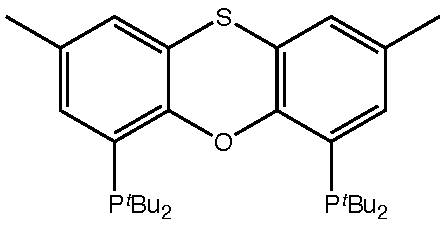
\includegraphics[scale=0.7]{structures/SP(tBu)2_ligand.pdf}
\end{center}
\end{structure}

\noindent \emph{s}-Butyllithium (\fixme{amount}) was added dropwise to a stirred solution of 2,8-Dimethylphenoxathiin (\fixme{amount}) and \gls{TMEDA} (\fixme{amount}) in diethyl ether (\fixme{amount}).  The resulting orange solution was stirred for \fixme{time} at room temperature.  Chlorodi-\emph{t}-butylphosphine was added dropwise and the reaction mixture was stirred for a further \fixme{time} resulting in a yellow solution with a white precipitate of lithium chloride.  The solvent was removed \emph{in vacuo} giving an orange oil.  This oil was taken up in dichloromethane \fixme{amount}, washed with water \fixme{amount}, dried over magnesium sulfate and solvent removed in vacuo.  The product was crystallised by dissolving in hot \emph{n}-propanol and cooling at \fixme{temperature} giving a pale yellow solid (\fixme{yield}).  This compound can be handled in the air for short periods however, should be stored under an inert atmosphere.
\fixme{IR, EA, 1H, 31P, 13C, MS}



\newpage{}
\subsection*{4,6-bis(di-\emph{tert}-butylphosphino)-10,10-dimethylphenoxasilin \\(\emph{t}-Bu-sixantphos)}

\begin{structure}
\begin{center}
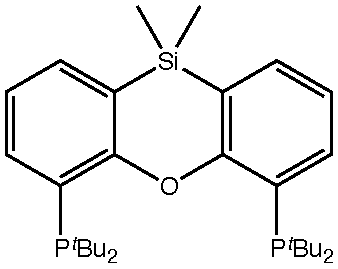
\includegraphics[scale=0.7]{structures/SiP(tBu)2_ligand.pdf}
\end{center}
\end{structure}

This compound was prepared similarly to \fixme{\emph{t}-Bu-thixantphos} from 10,10-dimethylphenoxasilin \fixme{amount}.  Yield:\fixme{yield}
\fixme{IR, EA, 1H, 31P, 13C, MS}



\newpage{}
\subsection*{\emph{t}-Bu-thixantphospalladiumdichloride, 2020} \fixme{check name}
\begin{structure}
\begin{center}
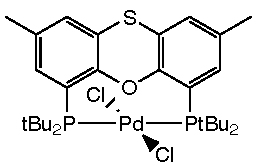
\includegraphics[scale=0.7]{structures/PdCl2(s(tBu)2)_complex.pdf}
\end{center}
\end{structure}

\fixme{IR, EA, 1H, 31P, 13C, MS}



\newpage{}
\subsection*{\emph{t}-Bu-thixantphossilverchloride, 3003} \fixme{check name}
\begin{structure}
\begin{center}
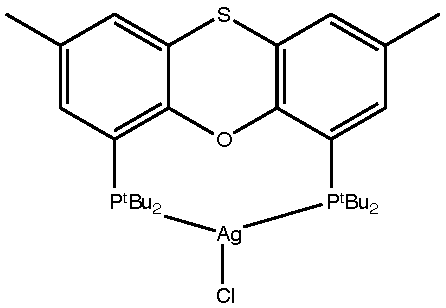
\includegraphics[scale=0.7]{structures/AgCl(s(tBu)2)_complex.pdf}
\end{center}
\end{structure}

$^1\textit{J} _{^{107}Ag}$

\fixme{IR, EA, 1H, 31P, 13C, MS}

%\subsection*{2,4-Di(carbomethoxy)-1,5-bis(\emph{p}-dimethylaminophenyl)-penta-1,4-dien-3-one}

%\begin{structure}
%\begin{center}
%\includegraphics[scale=1.2]{structures/dba436}
%\end{center}
%\end{structure}


%\noindent Dimethyl 1,3-acetonedicarboxylate (3.5~g, 0.02 mol), \textit{p}-di\-methy\-lamino\-benz\-aldehyde (6.0~g, 0.04 mol), piperidine (0.45~\cm, 4.6~mmol) and glacial acetic acid (0.30~\cm, 5.2~mmol) were combined in benzene (60~\cm) in a 250~\cm{} round bottom flask in the air.  The flask was equipped with a Dean-Stark trap to measure the volume of water being eliminated during the course of the reaction.  The trap was in turn equipped with a condenser, and the reaction mixture was heated under reflux for 1 day.  About 0.7~\cm{} of water were collected in the Dean-Stark trap indicating that the reaction was complete.  The solvent was removed \textit{in vacuo} to yield a dark red oil.  The oil was washed with petroleum ether several times then taken up in benzene.  The mixture was stirred at room temperature for several hours during which yellow crystalline solid precipitated out as the oil slowly dissolved.  The solid was filtered, washed with benzene and dried in the air
%(7.5~g, 86\%); 
%mp 124.5-124.8\degC{} (from benzene);
%(Found: C, 69.2; H, 6.5; N, 6.4. \ce{C25H28N2O5} requires C, 68.8; H, 6.5; N, 6.4\%);
%\numax(KBr)/\percm{} 1732, 1719, 1701, 1693, 1572, 1526, 1373, 1189 and 1158;  
%\dH(300~MHz; \ce{C6D6}; \ce{Me4Si}) 
%2.18 (6 H, s, \ce{NMe2}), 
%2.19 (6 H, s, \ce{NMe2}), 
%3.43 (3 H, s, OMe), 
%3.69 (3 H, s, OMe), 
%6.12 (2 H, d, \JHH{} 9.0, \textit{m}-H), 
%6.23 (2 H, d, \JHH{} 9.0, \textit{m}-H), 
%7.31 (2 H, d, \JHH{} 9.0, \textit{o}-H), 
%7.62 (2 H, d, \JHH{} 9.0, \textit{o}-H), 
%7.88 (1 H, s, CH=CH) and 
%8.32 (1 H, s, CH=CH);  
%\dC(75~MHz; \ce{C6D6}; \ce{Me4Si}) 
%39.15 (2 C, s, \ce{NMe2}), 
%39.17 (2 C, s, \ce{NMe2}), 
%51.8 (1 C, s, OMe), 
%52.0 (1 C, s, OMe), 
%111.8 (1 C, s, \textit{m}-\ce{C6H4}), 
%112.1 (1 C, s, \textit{m}-\ce{C6H4}), 
%120.9 (2 C, s, \ce{C6H4}), 
%121.2 (2 C, s, \ce{C6H4}), 
%132.5 (2 C, s, \textit{o}-\ce{C6H4}), 
%133.2 (2 C, s, \textit{o}-\ce{C6H4}), 
%143.7 (1 C, s, \textit{p}-\ce{C6H4}), 
%143.9 (1 C, s, \textit{p}-\ce{C6H4}), 
%166.5 (1 C, s, COO), 
%169.3 (1 C, s, COO) and 
%193.8 (1 C, s, CO);
%\textit{m/z} (ESI) 459.1000 (\MplusNa. \ce{C25H28N2O5Na} requires 459.1896).